\documentclass{beamer}
 
\usepackage{multirow}
\usepackage{longtable,booktabs,tabularx}
\usepackage[utf8]{inputenc}
\def\Put(#1,#2)#3{\leavevmode\makebox(0,0){\put(#1,#2){#3}}}
\usepackage{tikz}
\usetikzlibrary{arrows,shapes}
 \usepackage[sort, numbers]{natbib}
 \usepackage{siunitx}
\newcommand{\tikzmark}[1]{\tikz[remember picture] \node[coordinate] (#1) {#1};}
   
%Information to be included in the title page:
\title{Solar-Electric and Gas Powered, Long-Endurance UAV Sizing via Geometric Programming}
\author{Michael Burton and Warren Hoburg}
\institute{Massachusetts Institute of Technology}
\date{Feb 14, 2017}
 
\begin{document}
 
\frame{\titlepage}
 
\begin{frame}

\frametitle{Long-endurance UAV Applications}
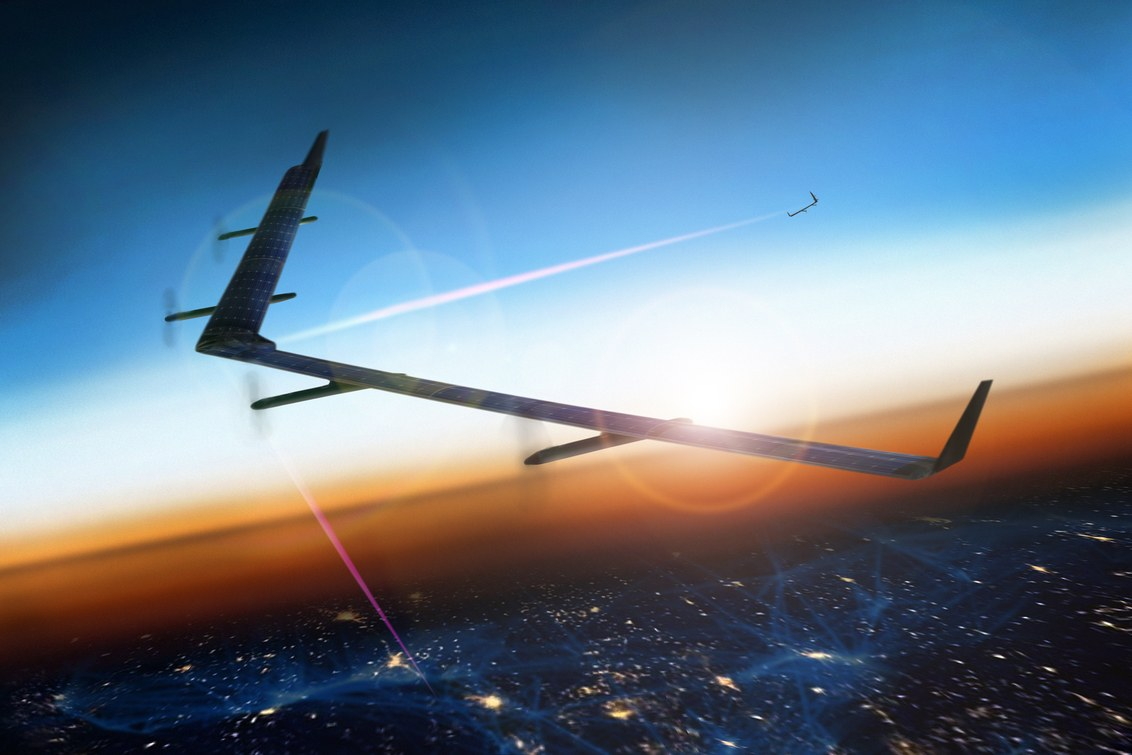
\includegraphics[height=4cm]{aquila.jpg}
    \pause
\Put(-150,90){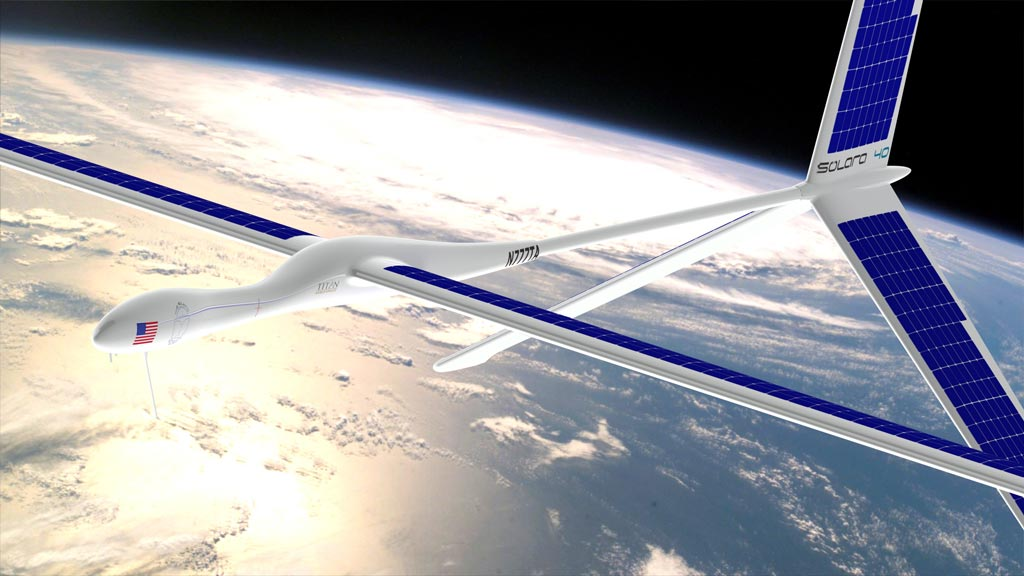
\includegraphics[height=4cm]{titan.jpg}}
    \pause
\Put(-130,80){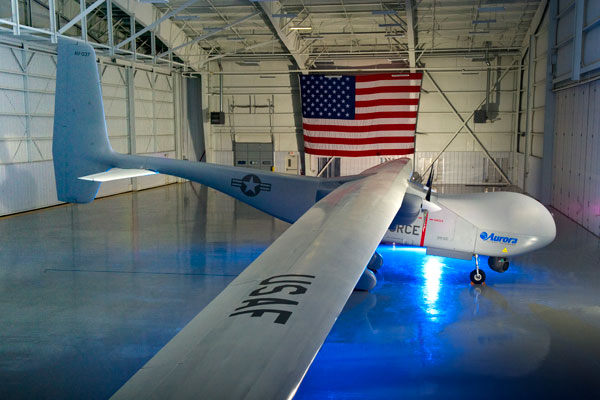
\includegraphics[height=4cm]{orion.jpg}}
    \pause
\Put(-100,70){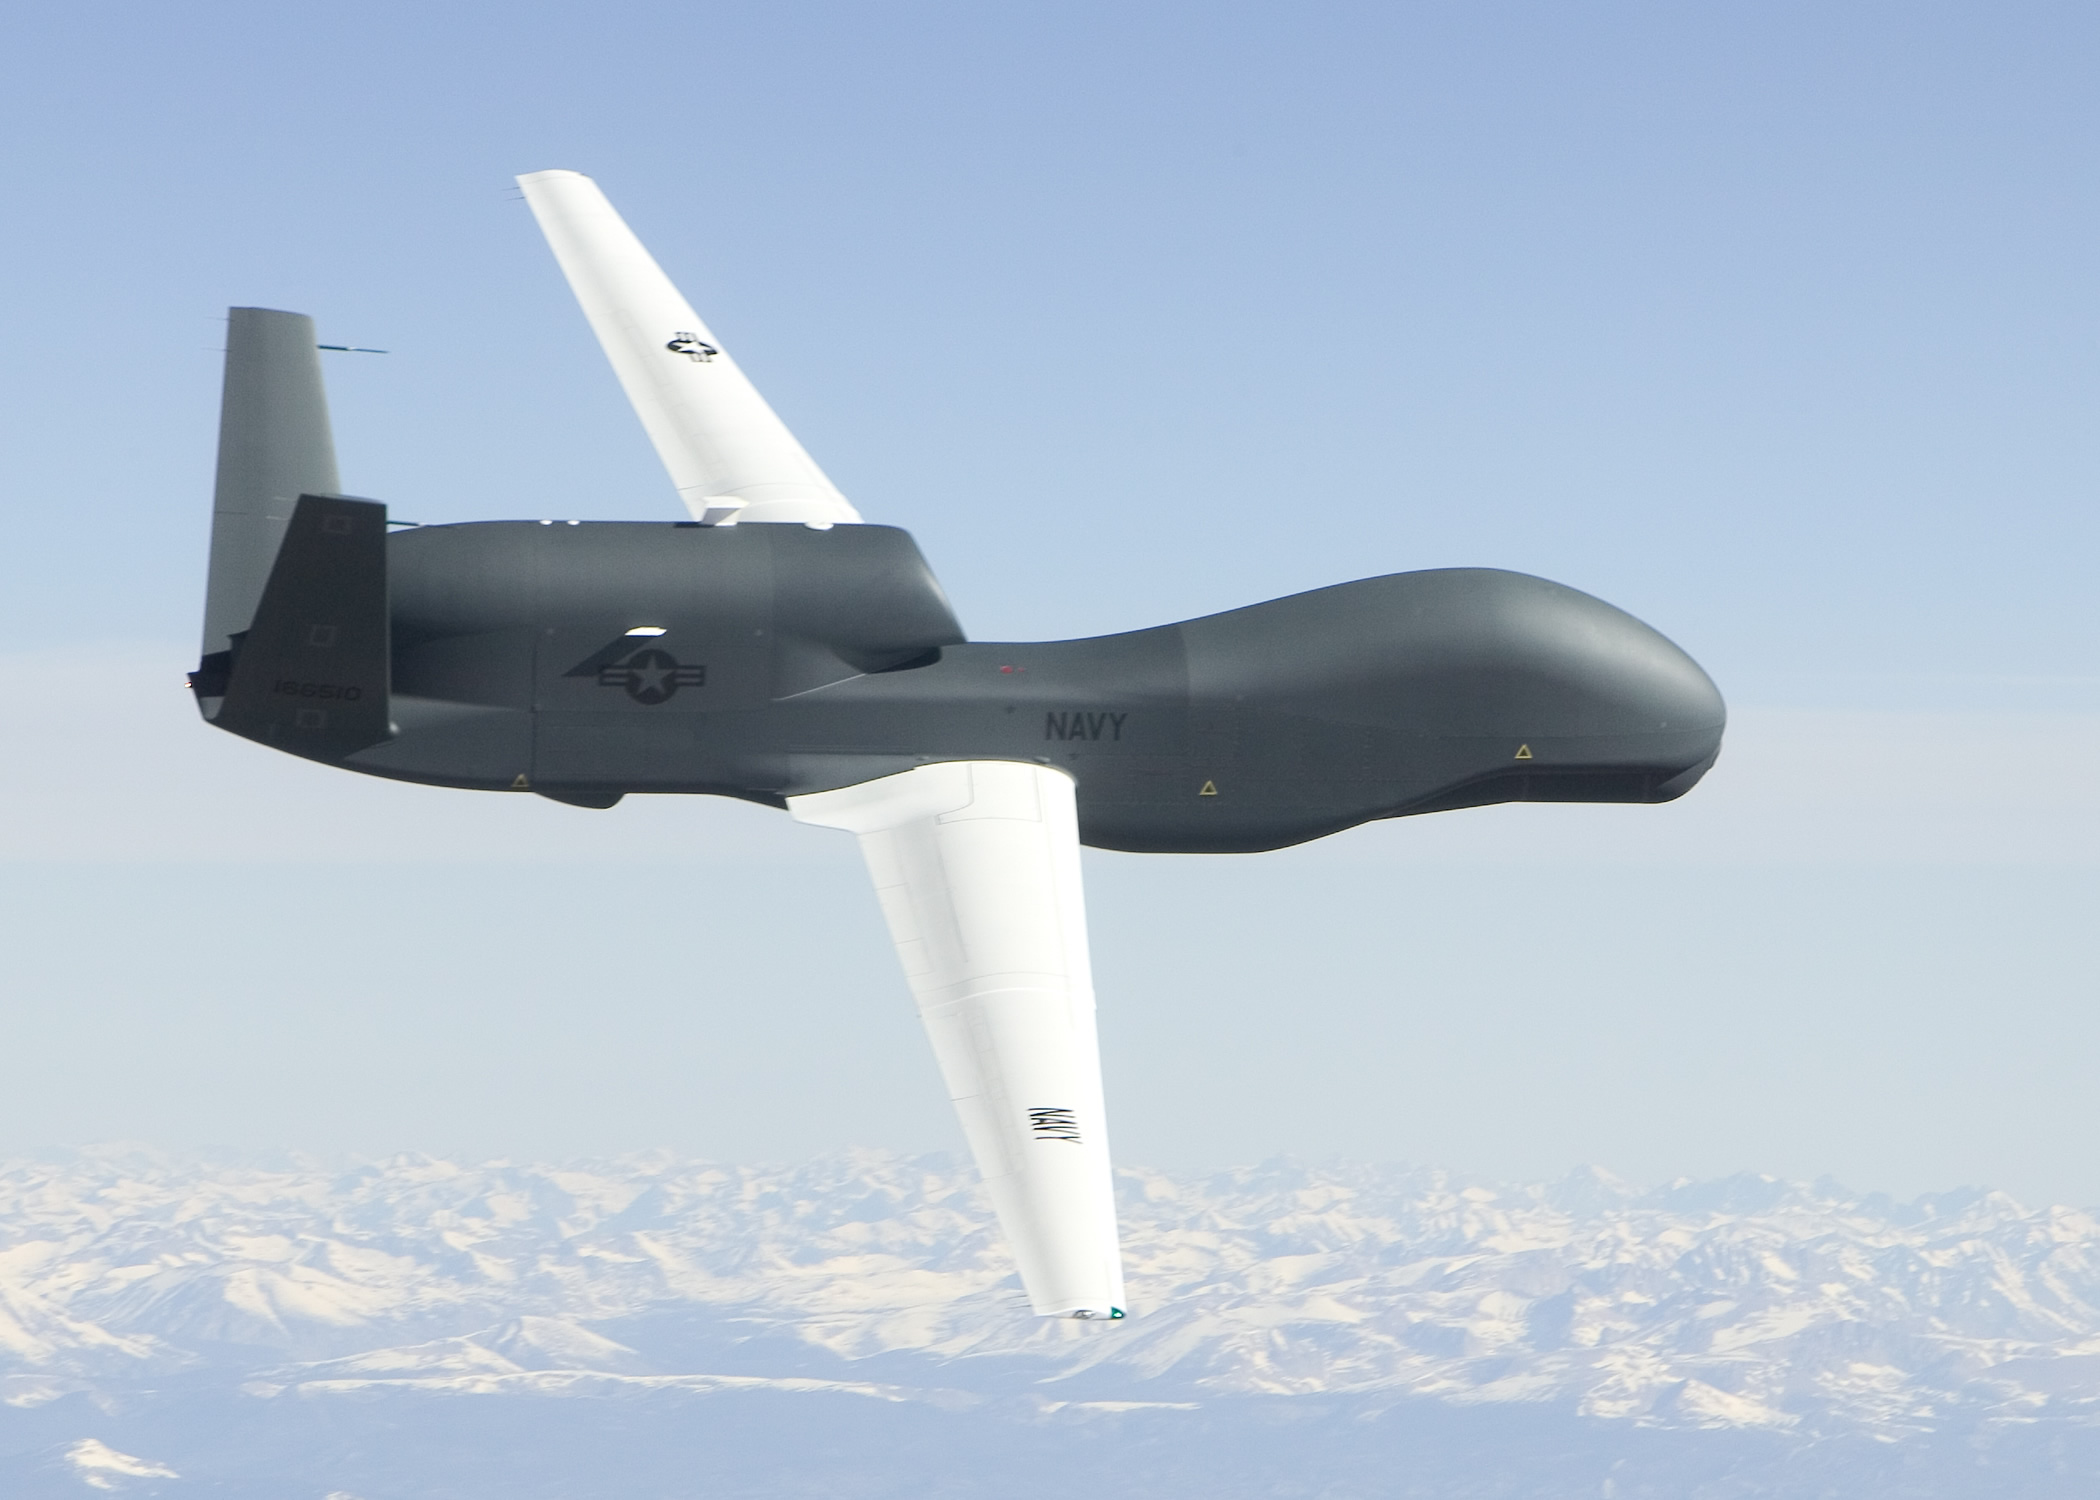
\includegraphics[height=4cm]{globalhawk.jpg}}
    \pause
\Put(-80,60){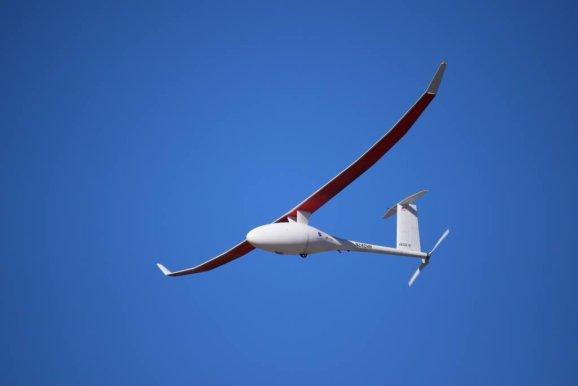
\includegraphics[height=4cm]{vanilla.jpg}}
    \pause
\Put(-60,60){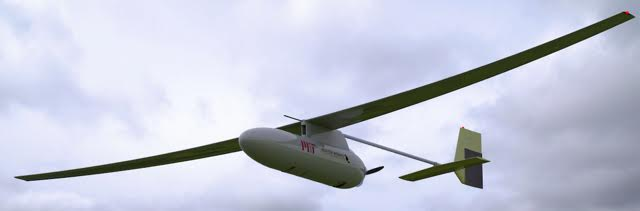
\includegraphics[height=3cm]{jho.jpeg}}

\end{frame}

\begin{frame}
    \frametitle{Problem}

    How do you hold a 10 lb payload in the air for a long time? \\~\\
    \pause
    Driving Requirements:
    \begin{itemize}
        \pause
        \item Payload ($W=10$ [lbs])
        \pause
        \item Endurance
            \begin{itemize}
                \pause
                \item Gas: time requirment (i.e. 5 days)
                \pause
                \item Solar: 24 hr availability (depends on solar flux)
                \end{itemize}
        \pause
        \item Station keeping ($V \geq V_{\text{wind}}$)
    \end{itemize}

\end{frame}

\begin{frame}
    \frametitle{Meeting the Requirements}

    \pause

    Solar flux = $f$(Latitude, Day) \\~\\

    \pause

    $ V_{\text{wind}} = f(\text{Lat}, \text{ Alt}, \text{ Percentile Wind Speed}, \text{ Day}) $

    \pause
    \begin{itemize}
        \item 90th Percentile Wind $\rightarrow V \geq V_{\text{wind}}$ 90\% of the time
        \end{itemize}


\end{frame}
 

\begin{frame}
    \frametitle{How Long Can You Fly?}

    \pause
    \begin{itemize}
        \item Gas: fuel 
            \pause
        \item Solar-electric: winter solstice \\~\\
    \end{itemize}

    \pause
    At 30$^{\circ}$ latitude:
    \begin{columns}
        \column{0.5\textwidth}
        \includegraphics[width=1.0\textwidth]{eirrvsmonth.pdf}
        
        \pause
        \column{0.5\textwidth}
        \includegraphics[width=1.0\textwidth]{windvsmonth.pdf}
    \end{columns}

\end{frame}

\begin{frame}
    \frametitle{Where Can You Fly?}
    
    \pause
    \begin{columns}
        \column{0.4\textwidth}
        \includegraphics[width=1.0\textwidth]{solaranglepic.pdf}
        
        \pause
        \column{0.6\textwidth}
        \begin{center}
        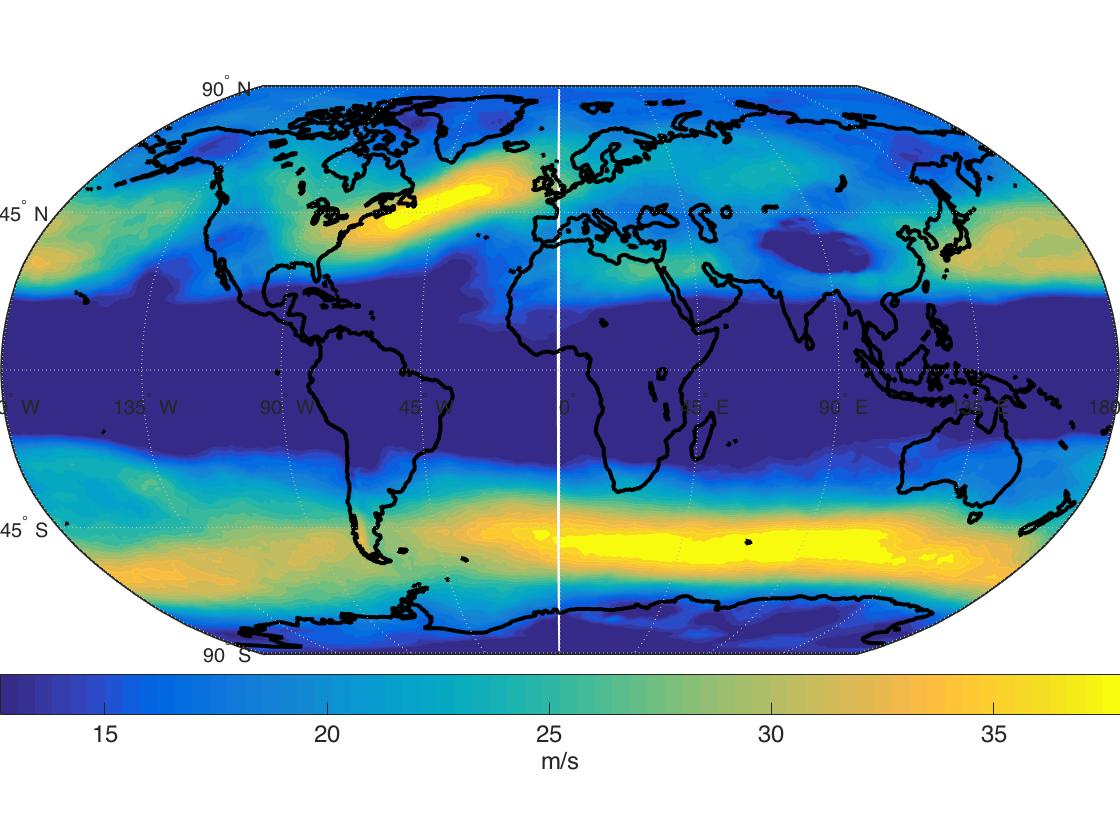
\includegraphics[width=1.0\textwidth]{worldwinds.jpg} \\
        90 percentile wind speeds in 2015
        \end{center}
    \end{columns}

\end{frame}

\begin{frame}
    \frametitle{Where Can You Fly?}

    \begin{center}
    \includegraphics[width=0.7\textwidth]{latvswind.pdf} \\
    \scriptsize
    80th, 90th, 95th Percentile Winds
    \end{center}

\end{frame}

\begin{frame}
    \frametitle{How High Can You Fly?}

    \pause
    Payload altitude requirement $\rightarrow h \geq h_{\text{min}}$ \\~\\

    \pause
    \begin{columns}
        \column{0.55\textwidth}
        \includegraphics[width=1.0\textwidth]{altvswind.pdf}

        \pause
        
        \column{0.45\textwidth}
        \begin{itemize}
            \item Gas: determined by payload
                \begin{itemize}
                    \item (5,000 - 25,000 ft)
                    \end{itemize}
                    \pause
            \item Solar-electric: optimized 
                \begin{itemize}
                    \item (55,000 - 70,000 ft)
                    \end{itemize}
                \end{itemize}
        
    \end{columns}

\end{frame}


\begin{frame}
    \frametitle{How to set up the problem?}

    \pause 
    \begin{columns}
        \column{0.6\textwidth}
        \includegraphics[width=1.0\textwidth]{simpleaircraft2.pdf}
        
        \column{0.4\textwidth}
        \begin{itemize}
            \pause
            \item Wind speeds
            \pause
            \item Solar energy
            \pause
            \item Endurance
            \pause
            \item Structural loads
            \pause
            \item Control authority
            \pause
            \item Aerodynamics
            \pause
            \item Powerplant
            \pause
            \item Weights \\~\\
            \end{itemize}
    \end{columns}
    
    \pause
    \begin{columns}
        \column{0.6\textwidth}
    \begin{center}
       number of unknowns
    \end{center}
    \begin{columns}
        \column{0.5\textwidth}
        \begin{center}
        Gas: 607 
        \end{center}
        
        \column{0.5\textwidth}
        \begin{center}
        Solar: 375
        \end{center}
        
    \end{columns}
        \column{0.4\textwidth}
    \end{columns}

\end{frame}

\begin{frame}
    \frametitle{Geometric Programming}
    \begin{itemize}
        \pause
        \item Non-linear optimization \\~\\
        \pause
        \item Can be solved extremely quickly ($\sim 0.1$ sec)\\~\\
        \pause
        \item Numerically stable \\~\\
        \pause
        \item Guaranteed global optimum \\~\\
        \pause
        \item No initial guess
        \end{itemize}
\end{frame}

\begin{frame}
    \frametitle{GP Form}

        \begin{align*}
            \text{minimize } &g_0(x) \\
            \text{subject to } &f_i(x) = 1, &i &= 1,\dots,m\\
                               &g_i(x) \leq 1, &i &= 1,\dots,n
        \end{align*}

        \begin{align*}
            f(\bold{x}) &= c x_1^{a_1} x_2^{a_2} \dotsm x_n^{a_n} , \\
            g(\bold{x}) &= \displaystyle\sum_{k=1}^K c_k x_1^{a_{1_k}} x_2^{a_{2_k}} \dotsm x_n^{a_{n_k}}.
        \end{align*}

\end{frame}

\begin{frame}
    \frametitle{Bag of Constraints}
    \pause
    \begin{columns}
        \column{0.5\textwidth}
    \begin{itemize}
        \scalebox{0.25}{\parbox{1.0\linewidth}{%
        \item Wind speed
        \begin{align*}
        V \geq V_{\text{wind}} \\
        \left(\frac{V_{\text{wind}}}{V_{\text{ref}}}\right)^{7.213} &\geq 2918\rho^{7.587}p_{\text{wind}}^{9.37} + \num{1.58d-10}\rho^{-6.074}p_{\text{wind}}^{60.421} \\
                                                                    &+ \num{4.05d-16}\rho^{-9.879}p_{\text{wind}}^{13.204} + 1048\rho^{6.33}p_{\text{wind}}^{46.232} 
\end{align*}
    
        \item Solar energy
        \begin{align*}
        (E/S)_{\text{sun}}  &\geq (E/S)_{\text{day}} + \frac{E_{\text{batt}}}{\eta_{\text{charge}}\eta_{\text{solar}} S_{\text{solar}}} \\
    E_{\text{batt}} &\geq \frac{P_{\text{oper}}t_{\text{night}}}{\eta_{\text{discharge}}} + (E/S)_{\text{twilight}} \eta_{\text{solar}} S_{\text{solar}} \\
    (P/S)_{\text{min}} &= \frac{P_{\text{oper}}}{\eta_{\text{solar}} S_{\text{solar}}} \\
    \eta_{\text{motor}} P_{\text{oper}} &\geq P_{\text{shaft}} + P_{\text{avionics}}\\
            (E/S)_{\text{twilight}}) &= 0.00315661 ((P/S)_{\text{min}})^{2.02484} \\
            (E/S)_{\text{day}} &= 14.1013((P/S)_{\text{min}})^{0.918619} \\
            S_{\text{solar}} & \leq f_{\text{solar}}S
        \end{align*}
        
    \item Breguet Endurance
        \begin{align*}
        \sqrt{W_i W_{i+1}} &= \frac{1}{2} \rho_i V_i^2 C_{L_i} S \\
        z_{bre_i} &\geq \frac{P_{\text{shaft}_i}t_i \text{BSFC} g}{\sqrt{W_i W_{i+1}}}\\
        \frac{W_{\text{fuel}_i}}{W_{i+1}} &\geq z_{bre_i} + \frac{z_{bre_i}^2}{2} + \frac{z_{bre_i}^3}{6} + \frac{z_{bre_i}^3}{24} 
        \end{align*} 
    \item Steady Level Flight
        \begin{align*}
            T &\geq \frac{1}{2} \rho V^2 C_D S\\
            W &= \frac{1}{2} \rho V^2 C_L S \\
            P_{\text{shaft}} &= \frac{TV}{\eta_{\text{prop}}}
        \end{align*}
        
    \item Aerodynamics
        \begin{align*}
            C_D &\geq C_{d_0} + c_{d_p} + \frac{C_L^2}{\pi e A} \\
        c_{d_p}^{3.72} &\geq 0.0247C_L^{2.49}Re^{-1.11} + 2.03e^{-7}C_L^{12.7}Re^{-0.338} + 6.35e^{10}C_L^{-0.243}Re^{-3.43} \nonumber \\
                       &+ 6.49e^{-6}C_L^{-1.9}Re^{-0.681} \\
        Re &= \frac{\rho V S/b}{\mu}
        \end{align*}

    \item Fuselage
        \begin{align*}
            \mathcal{V}_{\text{fuse}} &\geq \frac{W_{\text{fuel}}}{\rho_{\text{fuel}}} \\
            \mathcal{V}_{\text{fuse}} & \leq \frac{4}{3}\pi \frac{l_{\text{fuse}}}{2}R_{\text{fuse}}^2 \\
            3 \left( \frac{S_{\text{fuse}}}{\pi} \right)^{1.6075} &\geq 2(2l_{\text{fuse}}R_{\text{fuse}})^{1.6075} + (4R_{\text{fuse}}^2)^{1.6075} \\
            W_{\text{fuse}} &\geq S_{\text{fuse}} \rho_{A_{\text{cfrp}}} g \\
        D_{\text{fuse}} &\geq C_f k_{\text{fuse}} \frac{1}{2} \rho V^2 S_{\text{fuse}} \\
        C_f &\geq \frac{0.455}{Re^{0.3}}\\
            k_{\text{fuse}} &\geq 1 + \frac{60}{(l_{\text{fuse}}/2R_{\text{fuse}})^3} + \frac{(l_{\text{fuse}}/2R_{\text{fuse}})}{400}
        \end{align*}


}}
    \end{itemize}
    
    \column{0.5\textwidth}
    \begin{itemize}
        \scalebox{0.25}{\parbox{1.0\linewidth}{%
        \item Bending Model
        \begin{align*}
            \bar{q}(y) \equiv \frac{q(y)b}{N_{\text{max}}W_{\text{cent}}} &= \frac{2}{1+\lambda} \left( 1 + (\lambda - 1) \frac{2y}{b} \right) \\
            W_{\text{cent}} &\geq W_{\text{fuel}} + W_{\text{fuselage}} + W_{\text{engine}} + W_{\text{payload}} + W_{\text{empennage}} \\
            W_{\text{cent}} &\geq W_{\text{payload}} + W_{\text{motor}} + W_{\text{empennage}} \\
    \bar{q}(y) = \frac{q(y)b}{W_{\text{cent}}N_{\text{max}}} &\geq \bar{c}(y) \left[1 + \frac{c_{l_{\alpha}}}{C_L} \alpha_{\text{gust}} (y) \left(1 + \frac{W_{\text{wing}}}{W_{\text{cent}}} \right) \right] \\
            W_{\text{wing}} &\geq W_{\text{spar}} + W_{\text{skin}} \\
            W_{\text{wing}} &\geq W_{\text{spar}} + W_{\text{skin}} + W_{\text{batt}} + W_{\text{solar}} \\
            \alpha_{\text{gust}}(y) &= \tan^{-1}\left(\frac{V_{\text{gust}}(y)}{V} \right) \\
        \mathcal{S}_{i+1} &\geq \mathcal{S}_i + \frac{q_{i+1} + q_i}{2} \Delta y \\
        \mathcal{M}_{i+1} &\geq \mathcal{M}_i + \frac{\mathcal{S}_{i+1} + \mathcal{S}_i}{2} \Delta y \\
        \Theta_{i} &\geq \Theta_{i+1} + \frac{1}{2} \left(\frac{\mathcal{M}_i}{EI_i} + \frac{\mathcal{M}_{i-1}}{EI_{i-1}} \right) \Delta y \\
        w_{i} &\geq w_{i+1} + \frac{1}{2} (\Theta_i + \Theta_{i-1}) \Delta y \\
        I_i &\leq 2w_{\text{cap}_i}t_{\text{cap}_i}\left(\frac{h_{\text{cap}_i}}{2}\right)^2 \\
        c(y)\tau_t &\geq h_{\text{cap}_i} + 2t_{\text{cap}_i} \\
        c(y)\tau_w &\geq w_{\text{cap}_i} \\
        \Delta W_i &\geq \rho_{\text{cfrp}} w_{\text{cap}_i}t_{\text{cap}_i} \frac{b/2}{n-1}g \\
        W_{\text{spar}} &\geq 2 \sum\limits_{1}^{n-1} \Delta W_i 
        \end{align*}

    \item Empennage
        \begin{align*}
            W_{\text{skin}} & \geq 2 \rho_{A_{\text{cfrp}}} S g \\
            m &\geq \pi \rho_{\text{cfrp}} t_0 d l_{\text{h}} \left( 1 - \frac{1}{2} k\right) \\
            I_0 &\leq \pi t_0 d^3/8 \\
            \theta &\geq \frac{L_{\text{h}} l_{\text{h}}^2}{EI_0} \frac{1+k}{2} \\
            L_{\text{h}} &= \frac{1}{2} C_{L_{\text{h}}} \rho V^2 S_{\text{h}} \\
            V_{\text{h}} &= \frac{S_{\text{h}}l_{\text{h}}}{Sc} \\
            V_{\text{v}} &= \frac{S_{\text{v}}}{S} \frac{l_{\text{v}}}{b} \\
            W_{\text{h}}/m_{\text{fac}} &= \rho_{\text{foam}} \frac{S_{\text{h}}^2}{b_{\text{h}}} \bar{A} + g\rho_{A_{\text{cfrp}}} S_{\text{h}} \\
            W_{\text{v}}/m_{\text{fac}} &= \rho_{\text{foam}} \frac{S_{\text{v}}^2}{b_{\text{v}}} \bar{A} + g\rho_{A_{\text{cfrp}}} S_{\text{v}} \\
            D_{\text{h}} &\geq \frac{1}{2} c_{d_{\text{h}}} \rho V^2 S_{\text{h}} \\
            D_{\text{v}} &\geq \frac{1}{2} c_{d_{\text{v}}} \rho V^2 S_{\text{v}} \\
            c_{d_{\text{(v,h)}}}^{70.5599} &\geq \num{7.42688d-90} \left( \frac{Re_{\text{(v,h)}}}{\num{1d3}} \right)^{-33.0637}(100 \tau_{\text{(v,h)}})^{18.0419}  \nonumber \\
                         & + \num{5.02826d-163}\left(\frac{Re_{\text{(v,h)}}}{\num{1d3}}\right)^{-18.7959} (100\tau_{\text{(v,h)}})^{53.1879} \\
                         &+ \num{4.22901d-77}\left(\frac{Re_{\text{(v,h)}}}{\num{1d3}}\right)^{-41.1704} (100\tau_{\text{(v,h)}})^{28.4609} \nonumber \\
            Re_{\text{v}} &= \frac{V\rho S_{\text{v}}/b_{\text{v}}}{\mu} \\
            Re_{\text{h}} &= \frac{V\rho S_{\text{h}}/b_{\text{h}}}{\mu} 
        \end{align*}

}}
        \end{itemize}

\end{columns}

\end{frame}

\begin{frame}
    \frametitle{Weight Breakdown}

    \pause
    Gas Aircraft
    \begin{align*}
        \text{MTOW} &\geq W_{\text{structural}}  + W_{\text{payload}} + W_{\text{fuel}} + W_{\text{engine}} \\
        W_{\text{structural}} &\geq W_{\text{wing}} + W_{\text{boom}} + W_{\text{h}}+ W_{\text{v}} + W_{\text{fuse}}
    \end{align*}

    \pause
    Solar-electric Aircraft
    \begin{align*}
        \text{MTOW} &\geq W_{\text{structural}} + W_{\text{payload}} + W_{\text{solar}} + W_{\text{batt}} + W_{\text{motor}} \\
        W_{\text{structural}} &\geq W_{\text{wing}} + W_{\text{boom}} + W_{\text{h}}+ W_{\text{v}} \\
        W_{\text{solar}} &\geq \rho_{\text{solar}} S_{\text{solar}} g \\
        W_{\text{batt}} &\geq \frac{E_{\text{batt}}}{h_{\text{batt}}} g \\
        E_{\text{batt}} &= 350 \text{ [Whr/kg]}
    \end{align*}

\end{frame}

\begin{frame}

    \begin{center}
    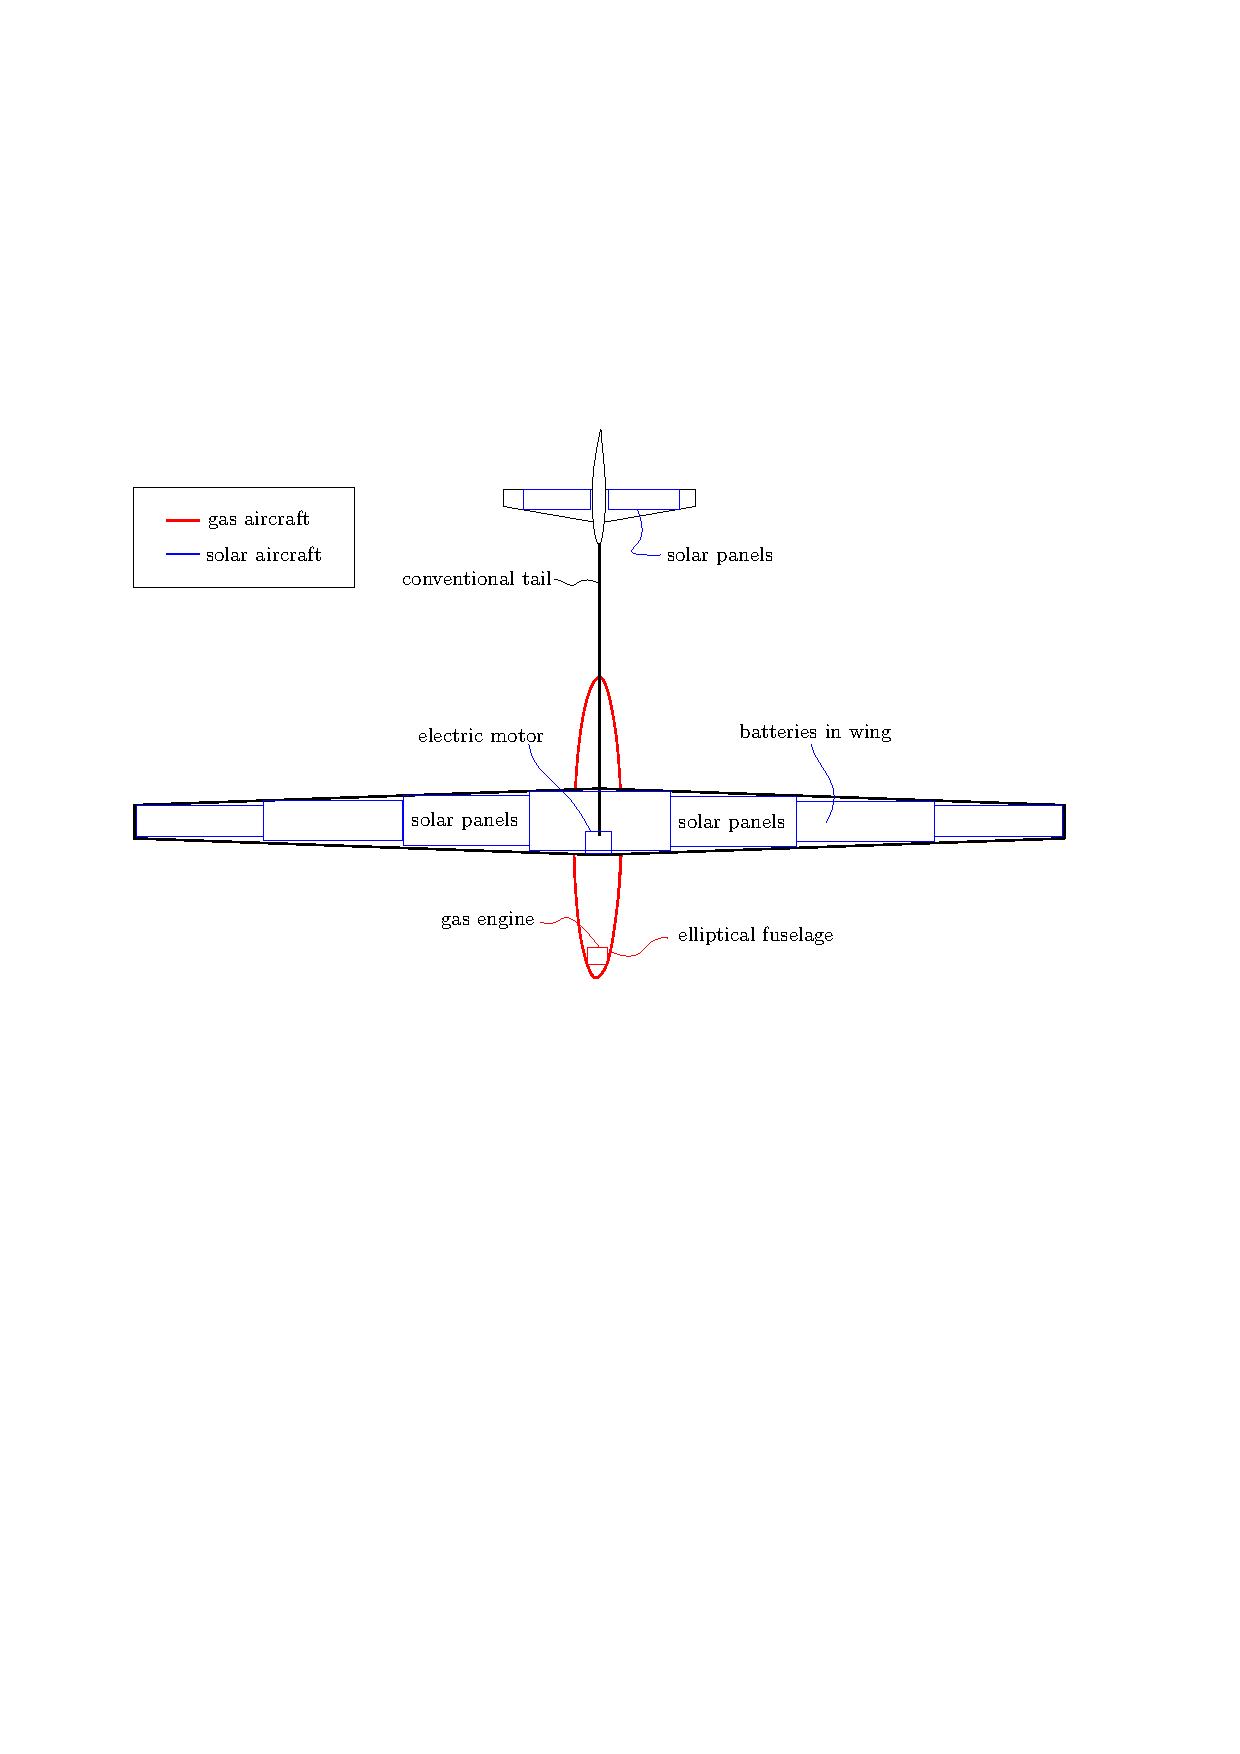
\includegraphics[width=1.0\textwidth]{simpleaircraft.pdf}
    \end{center}

\end{frame}

\begin{frame}
    \frametitle{Solar Energy Constraints}

    \begin{center}
    \includegraphics[width=0.7\textwidth]{lat30.pdf}
    \end{center}
    
    \pause
    \scriptsize
    \[ \begin{array}{rrl}
        \text{Solar Energy} : & (E/S)_{\text{sun}}  &\geq (E/S)_{\text{day}} + \frac{E_{\text{batt}}}{\eta_{\text{charge}}\eta_{\text{solar}} S_{\text{solar}}} \\
        \text{Battery Energy} : &E_{\text{batt}} &\geq \frac{P_{\text{oper}}t_{\text{night}}}{\eta_{\text{discharge}}} + (E/S)_{\text{twilight}} \eta_{\text{solar}} S_{\text{solar}} \\
        \text{Minimum operational solar power} : & (P/S)_{\text{min}} &= \frac{P_{\text{oper}}}{\eta_{\text{solar}} S_{\text{solar}}} 
    \end{array} \]

\end{frame}

\begin{frame}
    \frametitle{Wind Speed and Air Density Constraint}

    \pause
    \[ V \geq V_{\text{wind}} \]
        \pause
    \[P_{\text{shaft}} \sim V^3 \]

    \pause
    \begin{center}
    \includegraphics[width=0.6\textwidth]{windfitl35.pdf}
    \end{center}

\end{frame}


\begin{frame}
    \frametitle{Solar Aircraft Environmental Constraints}
    
    \begin{columns}
        \column{0.5\textwidth}
    \tiny
    \begin{itemize}
        \item Wind speed
        \begin{align*}
            V & \geq V_{\text{wind}} \\
        \left(\frac{V_{\text{wind}}}{V_{\text{ref}}}\right)^{\alpha} &\geq c_1 \rho^{e_{1,1}}p_{\text{wind}}^{e_{1,2}} + c_2 \rho^{e_{2,1}}p_{\text{wind}}^{e_{2,2}} \\
                                                                     &+ c_3 \rho^{e_{3,1}}p_{\text{wind}}^{e_{3,2}} + c_4 \rho^{e_{4,1}}p_{\text{wind}}^{e_{4,2}} \\
\end{align*}
    
        \item Solar energy
        \begin{align*}
        (E/S)_{\text{sun}}  &\geq (E/S)_{\text{day}} + \frac{E_{\text{batt}}}{\eta_{\text{charge}}\eta_{\text{solar}} S_{\text{solar}}} \\
    E_{\text{batt}} &\geq \frac{P_{\text{oper}}t_{\text{night}}}{\eta_{\text{discharge}}} + (E/S)_{\text{twilight}} \eta_{\text{solar}} S_{\text{solar}} \\
    (P/S)_{\text{min}} &= \frac{P_{\text{oper}}}{\eta_{\text{solar}} S_{\text{solar}}} \\
    \eta_{\text{motor}} P_{\text{oper}} &\geq P_{\text{shaft}} + P_{\text{avionics}}\\
            (E/S)_{\text{twilight}} &= c_1 (P/S)_{\text{min}}^{e_1} \\
            (E/S)_{\text{day}} &= c_2(P/S)_{\text{min}}^{e_2} \\
            S_{\text{solar}} & \leq f_{\text{solar}}S
        \end{align*}
    \end{itemize}
        
    \pause
    \column{0.5\textwidth}
        \includegraphics[width=1.0\textwidth]{latvswind.pdf} \\~\\
        \pause
        \includegraphics[width=1.0\textwidth]{solaranglepic.pdf}

\end{columns}

\end{frame}

\begin{frame}
    \frametitle{Lower Power Affects BSFC and Endurance}

    \pause
    \[ \text{Breguet Endurance}: t = \frac{W_{\text{ave}}}{P_{\text{shaft}}\text{BSFC}g} \ln{\left( \frac{W_{\text{initial}}}{W_{\text{final}}}\right)} \]
        
    \pause
    \begin{center}
    \includegraphics[width=0.7\textwidth]{powertobsfcfit.pdf}
    \end{center}

\end{frame}
        
\begin{frame}
    \frametitle{Engine Power Requirement Set at Top of Climb}

    \pause
    \scriptsize
    \[ \begin{array}{rrl}
            \text{Climb Rate}: & \dot{h} &\geq 100 \text{ [ft/min]} \\
            \text{Lapse Rate Definition}: &L_{\text{eng}}(h) &\equiv \frac{P_{\text{max}}}{P_{\text{SL-max}}} \\
            \text{Approxmiate Lapse Rate Equation}: & L_{\text{eng}}(h) &= 1 - \frac{0.035}{1000 \text{ [ft]}} h
    \end{array} \]

    \pause
    \begin{center}
    \includegraphics[width=0.7\textwidth]{powervsweightfit.pdf}
    \end{center}

\end{frame}

\begin{frame}
    \frametitle{Aerodynamics}

    \pause
    \[ C_D \geq C_{d_0} + c_{d_p} + \frac{C_L^2}{\pi e A} \]

    \begin{center}
    aircraft drag $\geq$ non-wing drag + wing profile drag + induced drag
    \pause
    \includegraphics[width=0.7\textwidth]{jho1polarfit1.pdf} \\
    \scriptsize
    JHO airfoil profile drag
    \end{center}
    
\end{frame}

\begin{frame}
    \frametitle{Wing Sizing for Load Cases}
      
    \begin{columns}
        \column{0.5\textwidth}
        \begin{center}
        Standard g-loading ($N_{\text{max}}$ = 5) \\~\\
        \end{center}
        
        \column{0.5\textwidth}
        \begin{center}
        Gust Loading ($N_{\text{max}}$ = 2) \\~\\
        \end{center}
    \end{columns}

    \pause

    \begin{columns}
        \column{0.5\textwidth}
        \includegraphics[width=1.0\textwidth]{gbending.pdf}
        
        \column{0.5\textwidth}
        \includegraphics[width=1.0\textwidth]{gustloaddiagram.pdf}
    \end{columns}
    
    \pause
    \begin{columns}
        \column{0.5\textwidth}
        \begin{center}
        Constrains gas powered aircraft \\~\\
        \end{center}
        
        \column{0.5\textwidth}
        \begin{center}
        Constrains solar-electric aircraft \\~\\
        \end{center}
    \end{columns}

    \pause
    \begin{table}[]
        \centering
        \begin{tabular}{cc}
            Architecture & Wing Loading [lbs/ft$^2$] \\ \hline
            Solar        & $\sim$ 1                        \\
            Gas          & $\sim$ 8                       
        \end{tabular}
    \end{table}
\end{frame}

\begin{frame}
    \frametitle{Discretized Beam}

    \pause
    \begin{center}
        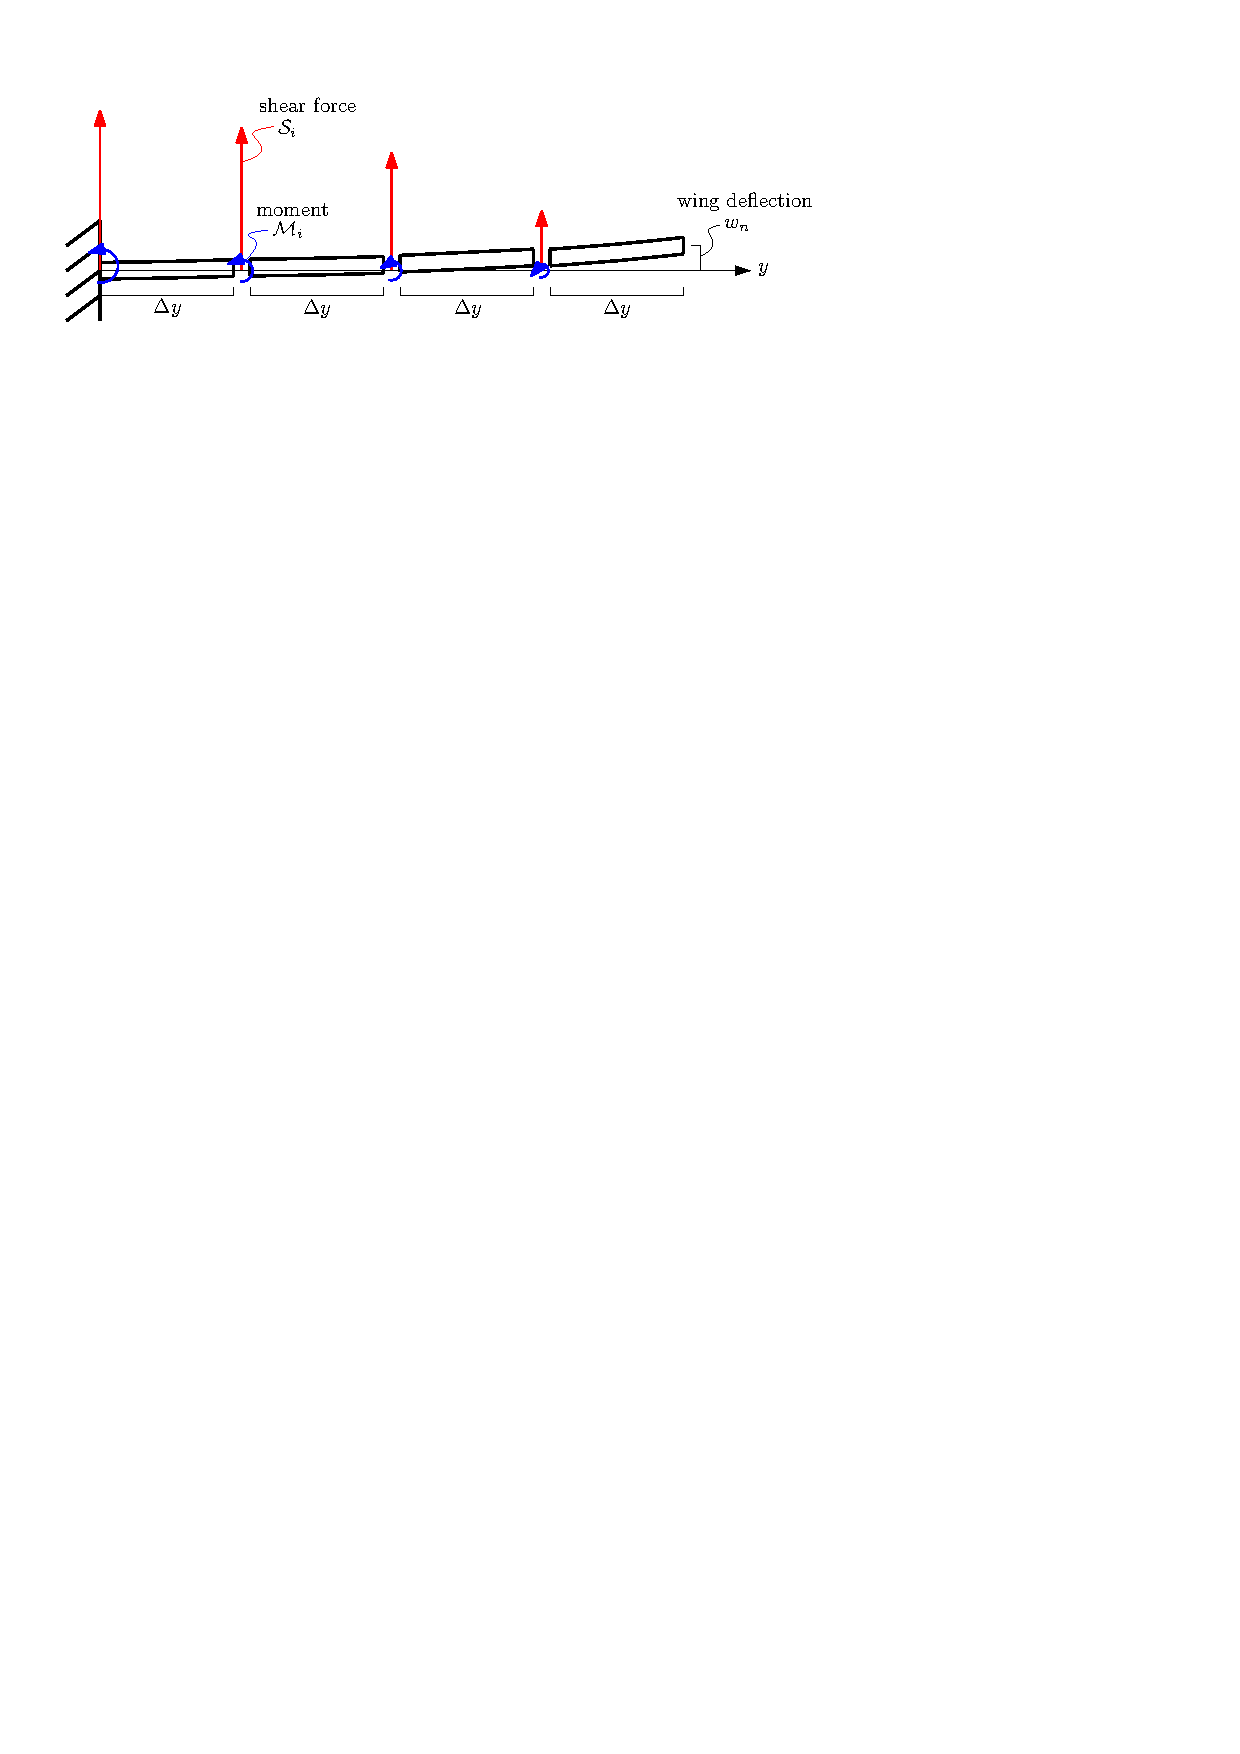
\includegraphics[width=0.8\textwidth]{disctbeam.pdf}
    \end{center}

    \pause
    \begin{align*}
        \mathcal{S}_{i+1} &\geq \mathcal{S}_i + \frac{q_{i+1} + q_i}{2} \Delta y \\
        \mathcal{M}_{i+1} &\geq \mathcal{M}_i + \frac{\mathcal{S}_{i+1} + \mathcal{S}_i}{2} \Delta y \\
        \Theta_{i} &\geq \Theta_{i+1} + \frac{1}{2} \left(\frac{\mathcal{M}_i}{EI_i} + \frac{\mathcal{M}_{i-1}}{EI_{i-1}} \right) \Delta y \\
        w_{i} &\geq w_{i+1} + \frac{1}{2} (\Theta_i + \Theta_{i-1}) \Delta y 
    \end{align*}
\end{frame}

\begin{frame}
    \frametitle{Cap Spar}

    \pause
    \begin{center}
    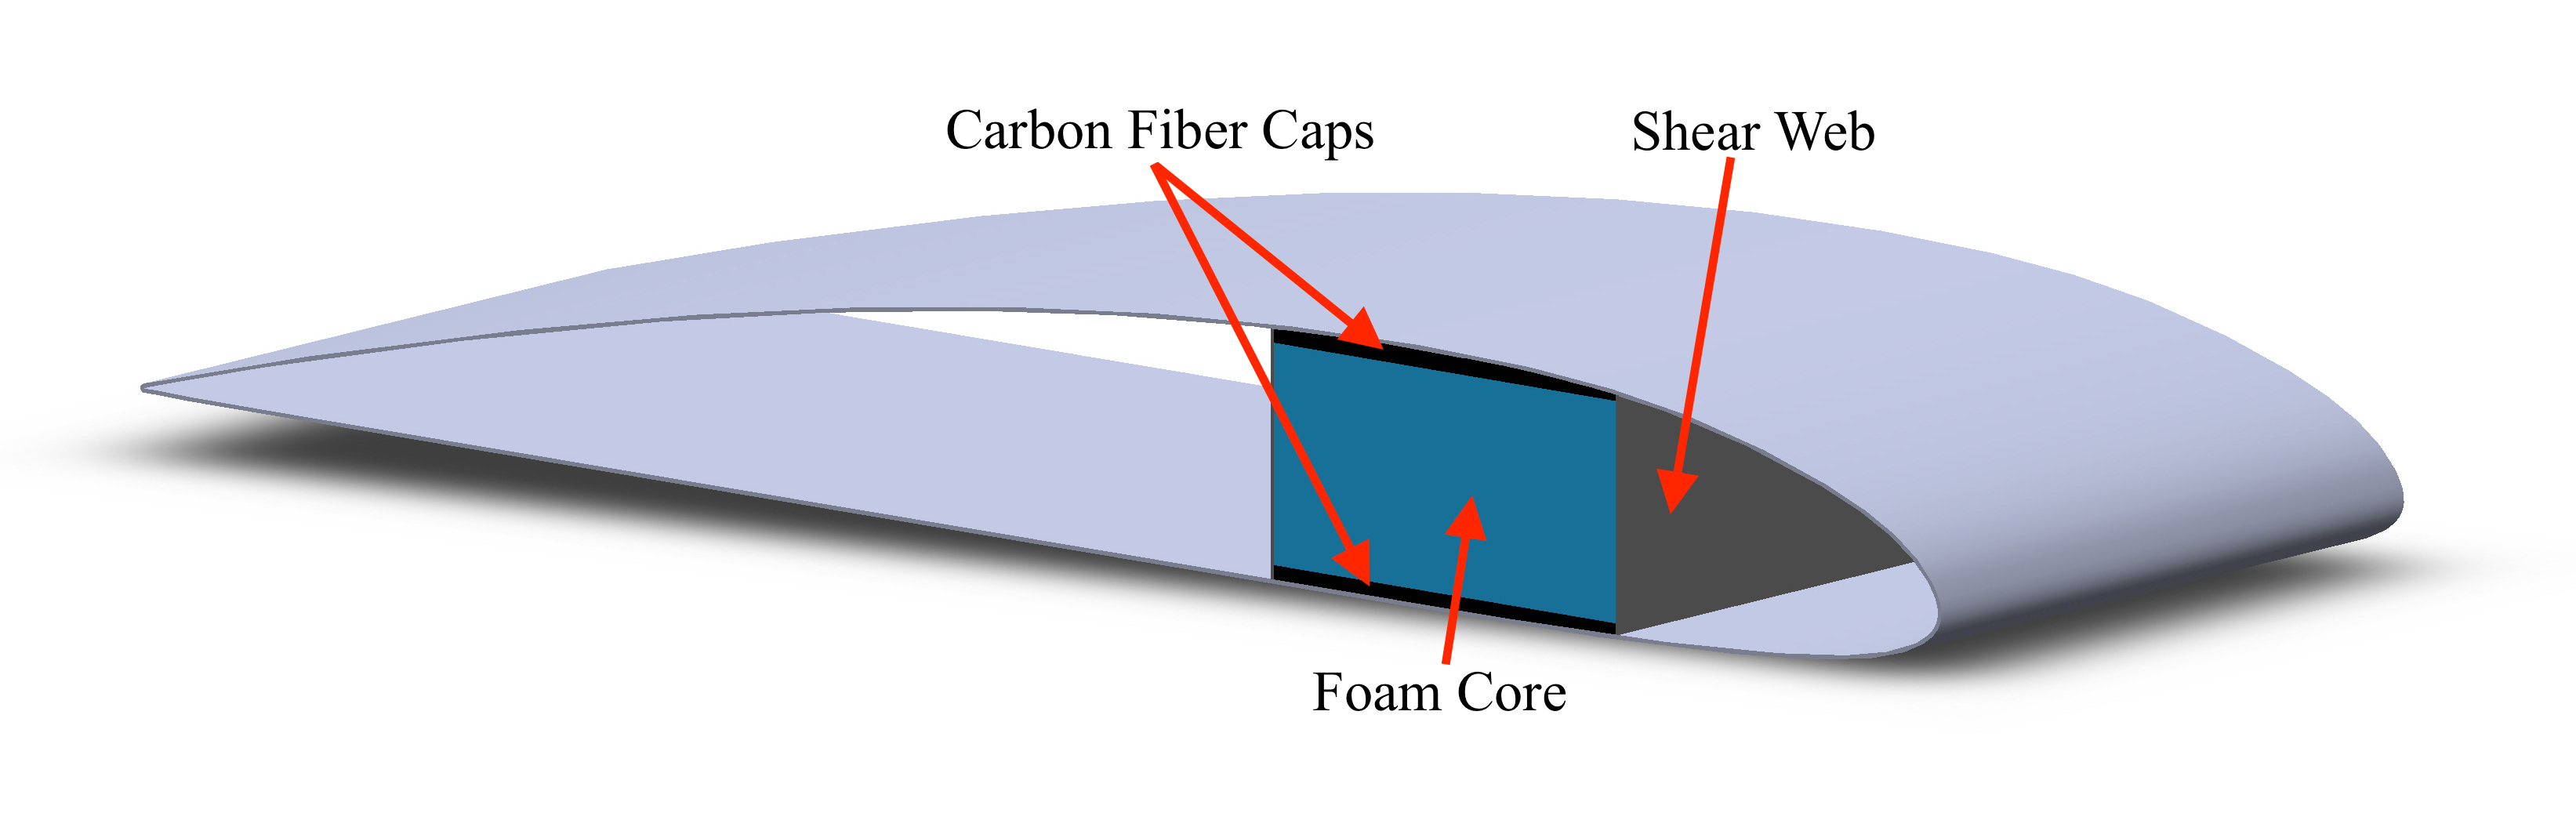
\includegraphics[width=0.8\textwidth]{capspar.jpg}
    \end{center}

    \pause
    \begin{columns}
        \column{0.5\textwidth}
        \begin{center}
        Dimensional Constraints
        \end{center}
        \column{0.5\textwidth}
        \begin{center}
        Moment and Deflection Constraints
        \end{center}
    \end{columns}
    
    \begin{columns}
        \column{0.5\textwidth}
        \begin{align*}
            I_i &\leq 2w_{\text{cap}_i}t_{\text{cap}_i}\left(\frac{h_{\text{cap}_i}}{2}\right)^2 \\
            c(y)\tau_t &\geq h_{\text{cap}_i} + 2t_{\text{cap}_i} \\
            c(y)\tau_w &\geq w_{\text{cap}_i} 
        \end{align*}

        \column{0.5\textwidth}
        \begin{align*}
            \sigma_{\text{cfrp}} &\geq \mathcal{M}_i \frac{h_{\text{cap}_i}+t_{\text{cap}_i}}{I_i}\\
            w_n &\leq w_{\text{max}}
        \end{align*}
        
    \end{columns}

\end{frame}



\begin{frame}
    \frametitle{Results}

    \pause
    \begin{center}
    \includegraphics[width=0.7\textwidth]{mtowvslat.pdf} \\
    Minimize MTOW
    \end{center}

\end{frame}

\begin{frame}
    \frametitle{Solar Feasibility}

    \pause
    \begin{center}
    \includegraphics[width=0.7\textwidth]{battsolarcontour.pdf} \\
    Minimizing battery specific energy for solar cell efficiency sweeps, 90th percentile wind speeds
    \end{center}

\end{frame}

\begin{frame}
    \frametitle{Maximizing Endurance for Globally Operational Aircraft}

    \pause
    \begin{center}
    \includegraphics[width=0.7\textwidth]{mtowvsendurance.pdf} \\
    Minimizing MTOW
    \end{center}

\end{frame}

\begin{frame}
    \frametitle{Changing Objectives on Solar Aircraft}

    \pause
    \begin{columns}
        \column{0.5\textwidth}
        \includegraphics[width=1.0\textwidth]{solarobjcomp.pdf}
        
        \column{0.5\textwidth}
        \includegraphics[width=1.0\textwidth]{solarobjcomp2.pdf}
    \end{columns}

\end{frame}

\begin{frame}
    \frametitle{Changing Structural Models on Solar Aircraft}


    \begin{center}
    \includegraphics[width=0.7\textwidth]{windaltoper0.pdf} \\
    \end{center}
    
    \[ \]
\end{frame}

\begin{frame}
    \frametitle{Changing Structural Models on Solar Aircraft}


    \begin{center}
    \includegraphics[width=0.7\textwidth]{windaltoper1.pdf} \\
    \end{center}
    
    \[ \]

\end{frame}

\begin{frame}
    \frametitle{Changing Structural Models on Solar Aircraft}


    \begin{center}
    \includegraphics[width=0.7\textwidth]{windaltoper.pdf} \\
    \end{center}
    
    \[ W_{\text{structural}} \geq \text{MTOW} f_{\text{structural}} \]

\end{frame}

\begin{frame}
    \frametitle{With and Without Wind Speed Constraint}

    \begin{center}
    \includegraphics[width=1.0\textwidth]{polarmission0.pdf} \\
    \end{center}

\end{frame}

\begin{frame}
    \frametitle{With and Without Wind Speed Constraint}

    \begin{center}
    \includegraphics[width=1.0\textwidth]{polarmission1.pdf} \\
    \end{center}

\end{frame}

\begin{frame}
    \frametitle{With and Without Wind Speed Constraint}

    \begin{center}
    \includegraphics[width=1.0\textwidth]{polarmission.pdf} \\
    \end{center}

\end{frame}

\begin{frame}
    \frametitle{Solar Aircraft Sensitivities: Objective = min(MTOW)}

    \pause
    Sensitivity of variable $x$ is $a$ \\
    1\% increase in $x \rightarrow$ $a\%$ increase in objective 
    \pause
    \begin{center}
        \scriptsize
        90th percentile winds, 30 degrees latitude
    \includegraphics[width=0.6\textwidth]{solarsensbar.pdf} 
    \end{center}

    \pause
    Break-even point = ratio of sensitivities

\end{frame}

\begin{frame}
    \frametitle{Gas Aircraft Sensitivities: Objective = min(MTOW)}
    
    \pause
    
    \begin{center}
        \scriptsize
        9 day endurance requirement
    \includegraphics[width=0.7\textwidth]{gassensbar.pdf} 
    \end{center}

\end{frame}

\begin{frame}
    \frametitle{Contributions}

    \begin{itemize}
        \pause
        \item Better understanding of long-endurance aircraft trade space \\~\\
        \pause
        \item Identified high level trade offs between architectures \\~\\
        \pause
        \item Proved that GP can be used to efficiently evaluate a complicated design space \\~\\
            \pause
        \item Built a working sizing model for gas and solar powered, long-endurance aircraft
        \end{itemize}

\end{frame}

\begin{frame}
    \frametitle{Configuration}
    
    \begin{columns}
        \column{0.5\textwidth}
        \begin{center}
        Component Weight
        \end{center}
        \column{0.5\textwidth}
        \begin{center}
        Component Drag
        \end{center}
    \end{columns}

    \begin{columns}
        \column{0.5\textwidth}
        \scriptsize
        \begin{align*}
        W_{\text{skin}} &\geq 2 \rho_{A_{\text{cfrp}}} S g \\
        W_{\text{boom}} &\geq \pi \rho_{\text{cfrp}} t_0 d l_{\text{h}}g \left( 1 - \frac{1}{2} k\right) \\
        W_{\text{h}}/m_{\text{fac}} &\geq \rho_{\text{foam}} \frac{S_{\text{h}}^2}{b_{\text{h}}} \bar{A} + g\rho_{A_{\text{cfrp}}} S_{\text{h}} \\
        W_{\text{v}}/m_{\text{fac}} &\geq \rho_{\text{foam}} \frac{S_{\text{v}}^2}{b_{\text{v}}} \bar{A} + g\rho_{A_{\text{cfrp}}} S_{\text{v}} \\
            W_{\text{fuse}} &\geq S_{\text{fuse}} \rho_{A_{\text{cfrp}}} g
        \end{align*}
        \column{0.5\textwidth}
        \scriptsize
        \begin{align*}
        D_{\text{boom}} &\geq \frac{1}{2} C_f \rho V^2 l_{\text{h}}\pi d \\
        D_{\text{fuse}} &\geq C_f k_{\text{fuse}} \frac{1}{2} \rho V^2 S_{\text{fuse}} \\
        C_f &\geq \frac{0.455}{Re^{0.3}} \\
        D_{\text{h}} &\geq \frac{1}{2} c_{d_{\text{h}}} \rho V^2 S_{\text{h}} \\
        D_{\text{v}} &\geq \frac{1}{2} c_{d_{\text{v}}} \rho V^2 S_{\text{v}} 
        \end{align*}
    \end{columns}

\end{frame}

\begin{frame}
    \frametitle{Percentile Wind Speed}
    
    \pause
    \begin{columns}
        \column{0.5\textwidth}
        \includegraphics[width=1.0\textwidth]{Boston_dec_2015.pdf}
    
        \column{0.5\textwidth}
        \includegraphics[width=1.0\textwidth]{Boston_dec_2015auto.pdf}
    \end{columns}

    \begin{center}
    Wind speeds in Boston, December 2015 at 60,000 ft. 
    \end{center}
    
\end{frame}

\end{document}
